%%%%%%%%%%%%%%%%%%%
%% KAPITEL Intro %%
%%%%%%%%%%%%%%%%%%%
%% JONAS         %%
%%%%%%%%%%%%%%%%%%%
\section{Einführung}

\gls{sap} \gls{byd} ist eine \gls{erp} \gls{ondemand} Cloudlösung. Die Nutzung wird monatlich bezahlt. Dadurch können Nutzerlizenzen dynamisch erworben werden und der Kunde bezahlt immer nur so viel, wie er muss.

\gls{byd} ist preiswert und skalierbar. Die Software wird innerhalb weniger Wochen bereitgestellt. Außerdem wird das System direkt bei \gls{sap} vor Ort im Rechenzentrum gehostet, sodass der Kunde keine weiteren IT-Investitionen tätigen muss.

\gls{byd} enthält alle nötigen vorkonfigurierten Geschäftsprozesse, von Verwaltung der Kundenbeziehungen, Materialbeschaffung und Lieferkettenverwaltung, bis hin zu Rechnungswesen und Werbeplanung. Trotzdem verliert der Kunde kaum Flexibilität gegenüber den etablierten \gls{sap}-Lösungen, wie \gls{zb} \gls{sap} Business One (siehe \ref{sec:business-one}).

Für Installation, Wartung und Aktualisierung der Lösung sorgt das integrierte Betriebsmodell. Alle Betriebskosten, die durch ein Vor-Ort System entstehen sind also im Preis einbegriffen. Damit kann sich der Kunde vollständig auf sein Kerngeschäft konzentrieren.

\gls{sap} \gls{byd} wird über eine sichere Internetverbindung und einen Webbrowser als dynamische Website aufgerufen. Somit können Mitarbeiter von überall auf ihren Arbeitsplatz zugreifen und müssen weder vor Ort im Büro sein oder sich anderweitig ins Firmennetz einwählen.

\subsubsection{Vorteile von ByD}

\begin{itemize}
\item Business ByDesign vereinigt alle Vorteile einer modernen Unternehmensanwendung, bei minimalen Anforderungen an die IT
\item SAP Business ByDesign greift auf bewährte Geschäftsvorfälle zu, die umgehend einsatzbereit sind
\item Der Kunde nutzt automatisch stets die aktuellste Softwareversion
\item SAP Business ByDesign schont die Investition für eine eigene IT-Infrastruktur, durch ein skalierbares Mietmodell
\item Wechselnde Geschäftsanforderungen gehen mit der Nutzung der Softwarebereiche Hand in Hand
\end{itemize}
\cite{itelligence}

%%%%%%%%%%%%%%%%%%%%%%%%%%%%%%%%
%% KAPITEL Benutzeroberfläche %%
%%%%%%%%%%%%%%%%%%%%%%%%%%%%%%%%
%% JONAS                      %%
%%%%%%%%%%%%%%%%%%%%%%%%%%%%%%%%
\section{Benutzeroberfläche}

\gls{byd} ist in verschiedene WorkCenter unterteilt, die jeweils einen bestimmten Zweck erfüllen.

\begin{figure}[H]
	\begin{center}
	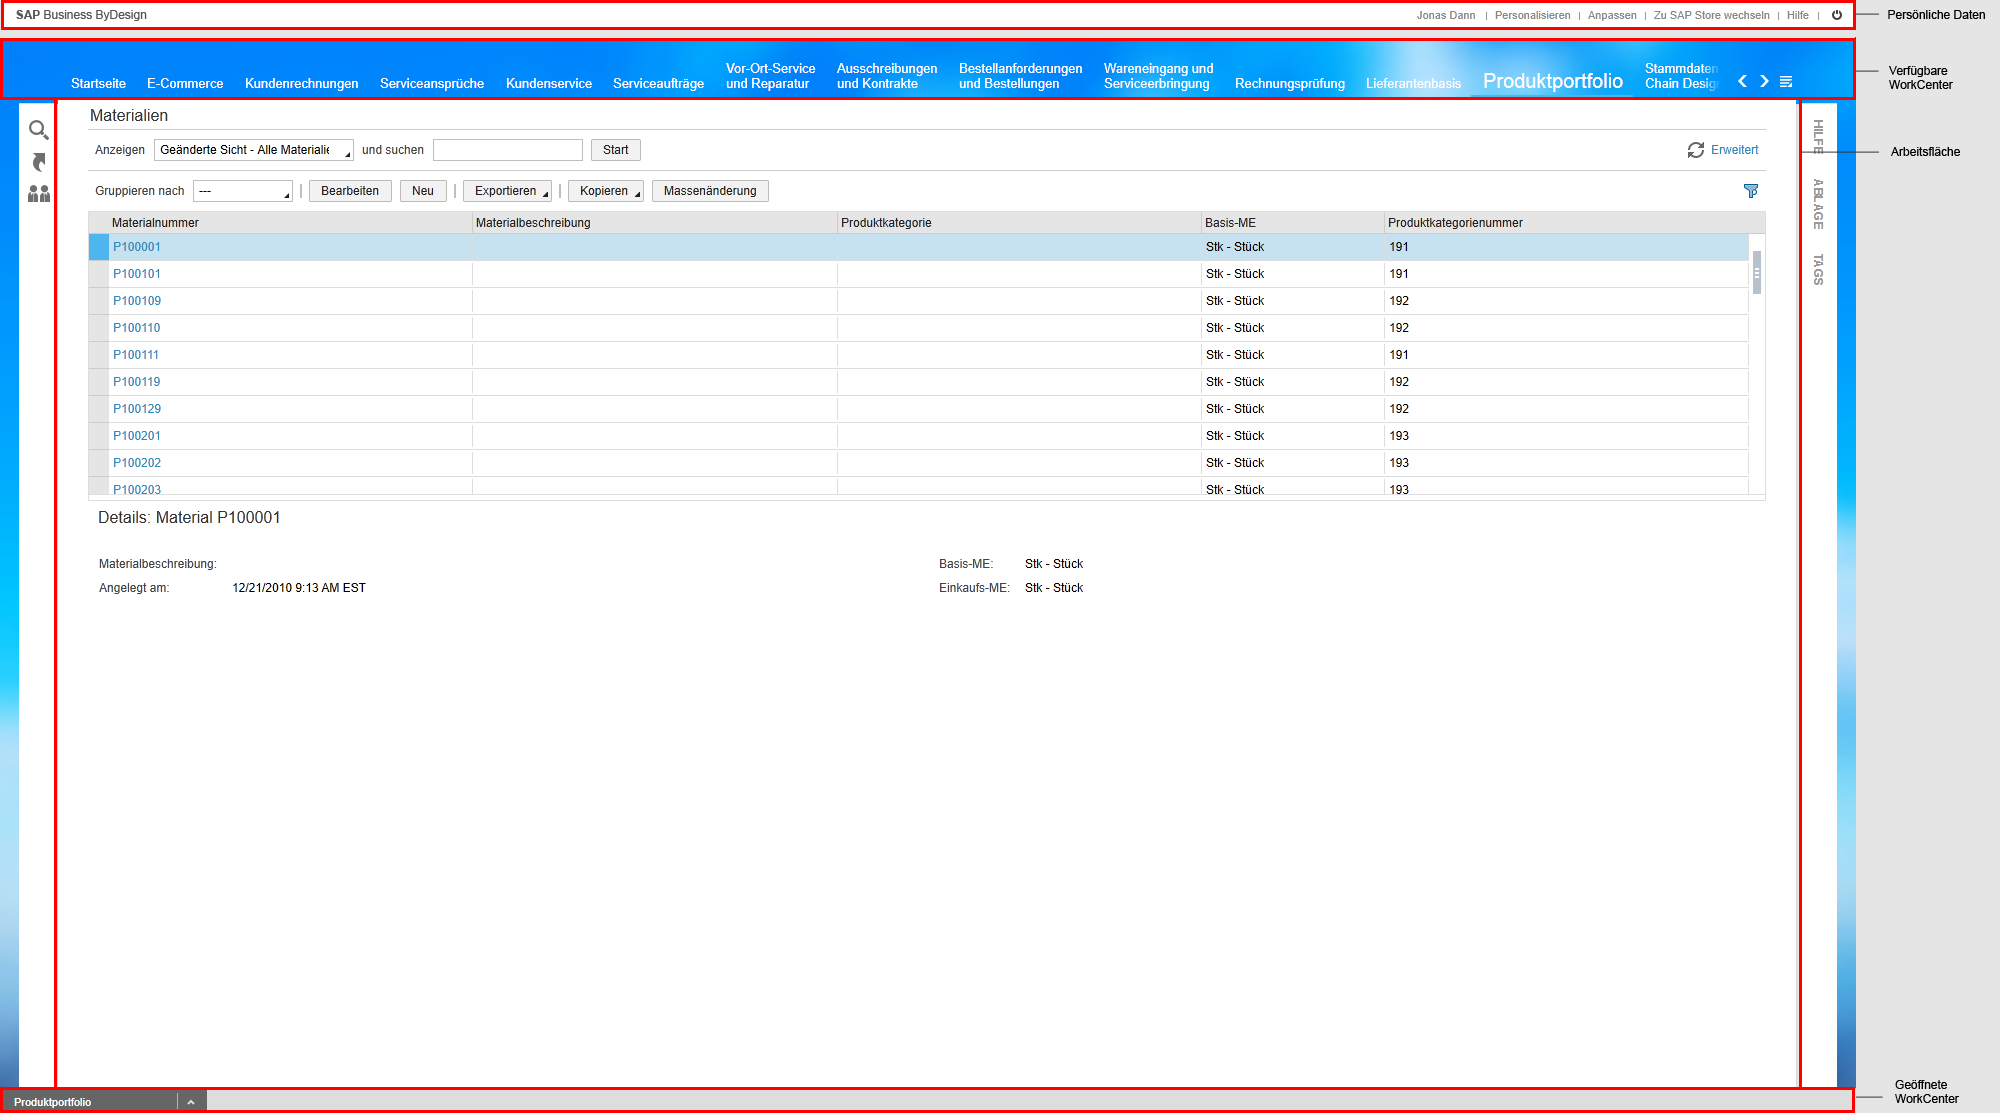
\includegraphics[width=1.0\textwidth]{grafiken/ByDesign-Ubersicht.png}
	\caption{ByDesgin Übersicht}
	\vspace{-10pt}
	\label{abb:byd-overview}
	\end{center}
\end{figure}

\subsubsection{Persönliche Daten}

Hier kann der Mitarbeiter seine Daten, wie \gls{zb} Telefonnummer oder E-Mail, einstellen und sein \gls{byd} konfigurieren.

\subsubsection{Verfügbare WorkCenter}

In dieser Sektion der Anzeige kann der User die verschiedenen, für ihn verfügbaren WorkCenter auswählen. Diese werden dann unten im "Geöffnete WorkCenter" Bereich geöffnet. So kann der Benutzer zwischen mehreren WorkCentern wechseln.

\subsubsection{Arbeitsfläche}

Hier werden die eigentlichen Inhalte des Webinterfaces angezeigt. Wenn der Beispielworkflow durchgespielt wird, werden auch nur noch diese Ausschnitte des Bildschirms gezeigt.

\subsubsection{Geöffnete WorkCenter}

Im Bereich "Geöffnete WorkCenter" sieht der Mitarbeiter alle WorkCenter, die er im Moment geöffnet hat.

%%%%%%%%%%%%%%%%%%%%%%%%%%%%%%
%% KAPITEL Beispielworkflow %%
%%%%%%%%%%%%%%%%%%%%%%%%%%%%%%
%% JONAS                    %%
%%%%%%%%%%%%%%%%%%%%%%%%%%%%%%
\section{Beispielworkflow}

\subsection{Vorstellung des Workflows}
\label{sec:byd-bsp-vorstellung}
% Schulungsworkflow beschreiben (anwendersicht)

\subsubsection{Szenario}

Der Verkaufsbereichsleiter unserer Firma hat auf einer Technologiemesse ein innovatives Produkt. Er würde gerne einen neuen Solarboiler in das Produktportfolio der Firma aufnehmen. Die Nachfrage nach Innovation ist sehr groß.

\subsubsection{Aufgabe des Mitarbeiters}

\begin{enumerate}
 \item Wir müssen in einem Katalog oder elektronischen Marktplatz einen Zulieferer für das gewünschte Produkt finden.
 \item Danach müssen wir den günstigsten Zulieferer finden, der gleichzeitig auch eine hohe Verfügbarkeit gewährleisten kann.
 \item Wenn wir ein passendes Produkt gefunden haben müssen wir dieses in \gls{sap} \gls{byd} einfügen und ihm eine Produktkategorie zuordnen.
 \item Währenddessen müssen alle wichtigen Daten über das Produkt in das System eingepflegt werden.
 \item Als Letztes müssen wir den Zulieferer für das neue Material im \gls{byd} einfügen.
 \end{enumerate}

\subsection{Umsetzung des Workflows}
\label{sec:byd-bsp-umsetzung}
% technische sicht, "`klickbares"' howto

\subsubsection{Produktsuche}

Im ersten Schritt suchen wir uns ein Produkt und einen Zulieferer auf der Website Alibaba\footnote{\url{alibaba.com}}. Auf dieser Website können kleine Unternehmer ihre Produkte zum Verkauf anbieten. Im Moment sind über 2 Millionen Zulieferer registriert.

Für unser Beispiel verwenden wir den SunSurf SC-IP01\footnote{\url{http://www.alibaba.com/product-detail/SunSurf-SC-IP01-solar-boiler-system_627442099.html?s=p}} Solar Boiler. Dieser kostet zwischen 400 und 500 USD(\$) und muss mindestens zu 15 Stück bestellt werden. Der Zulieferer kann maximal 5000 Stück im Monat liefern.

\subsubsection{Produkt im System anlegen}

Im WorkCenter "`Produktportfolio"' können wir nun die Daten des SunSurf SC-IP01 unter einem neuen Material abspeichern. Dazu klicken wir auf "`Produkte nach Materialien"' und dann auf "`Neu"'. In diesem Formular geben wir nun die Daten den Solar Boilers an:

\begin{figure}[H]
	\begin{center}
	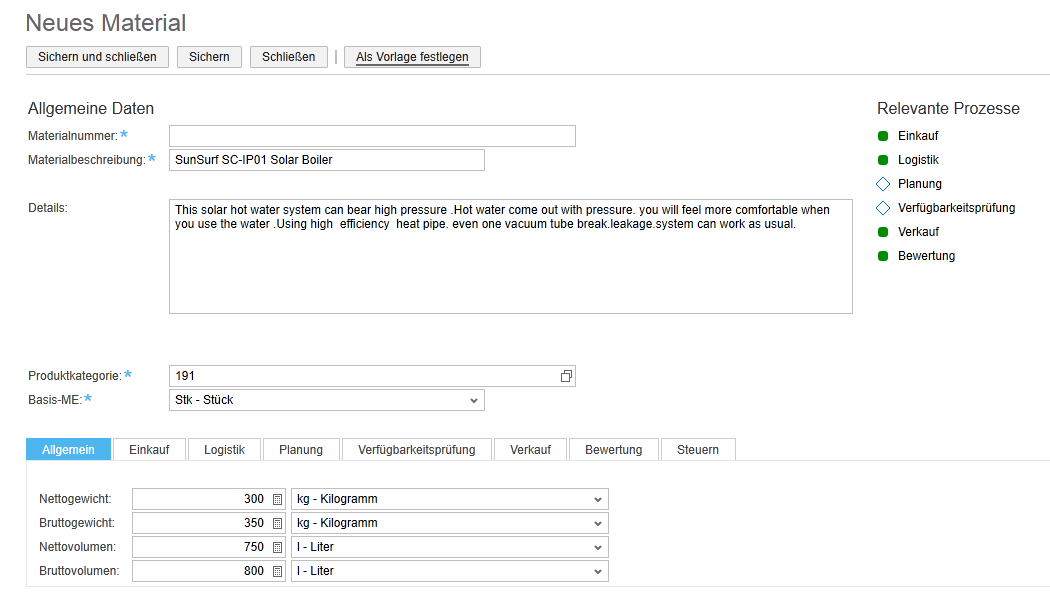
\includegraphics[width=1.0\textwidth]{grafiken/ByDesign-HowTo-1.png}
	\caption{Neues Material anlegen}
	\vspace{-10pt}
	\label{abb:byd-newmaterial}
	\end{center}
\end{figure}

Nachdem wir auf "`Sichern und schließen"' geklickt haben wurde unser Material erfolgreich angelegt.

\subsubsection{Zulieferer anlegen}

Im WorkCenter "`Lieferantenbasis"' unter "`Lieferanten"' können wir nur einen neuen Zulieferer anlegen. Dazu klicken wir wieder auf "`neu"'. In diesem Formular geben wir nun die Daten des Zulieferers ein:

\begin{figure}[H]
	\begin{center}
	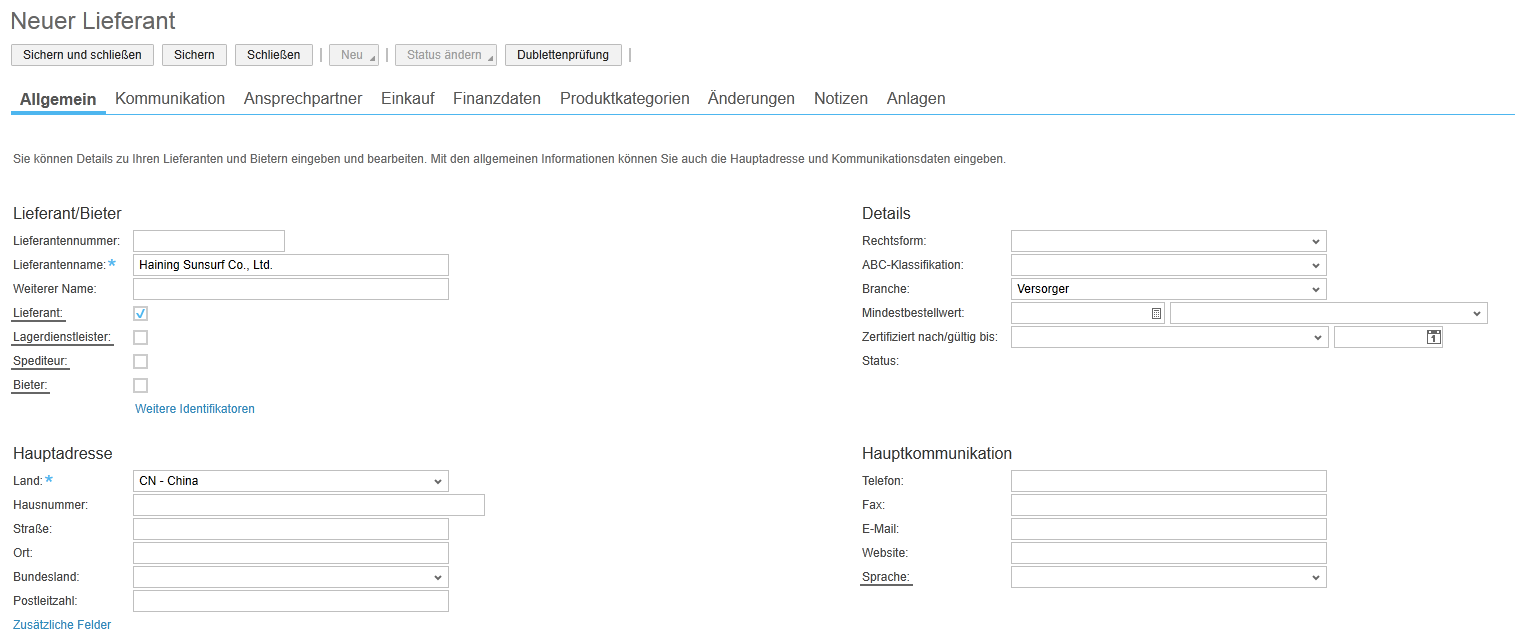
\includegraphics[width=1.0\textwidth]{grafiken/ByDesign-HowTo-2.png}
	\caption{Neuen Zulieferer anlegen}
	\vspace{-10pt}
	\label{abb:byd-newsupplier}
	\end{center}
\end{figure}

Nachdem wir auf "`Sichern und schließen"' geklickt haben wurde unser Zulieferer erfolgreich angelegt.

%%%%%%%%%%%%%%%%%%%%%
%% KAPITEL Grenzen %%
%%%%%%%%%%%%%%%%%%%%%
%% JONAS           %%
%%%%%%%%%%%%%%%%%%%%%
\section{Grenzen von ByD}

Trotz der vielseitigen Vorteile von \gls{byd} stößt auch diese Lösung, wie alle anderen, an ihre Grenzen.

\subsubsection{Vordefinierte Geschäftsprozesse}

Durch die Idee hinter \gls{byd}, eine vorkonfigurierte On-Demand Unternehmensmanagement Applikation bereitzustellen, weißt es Nachteile gegenüber den anderen \gls{sme}-Lösungen im Bereich Customizing auf. So kann \gls{byd} nicht beliebig eingestellt werden.

\subsubsection{Module}

Da \gls{byd} in Form von Modulen zusammengestellt wird bekommt der Kunde unausweichlich auch Funktionalität, die er gar nicht benötigt und bezahlt für unnötige Anwendungsbestandteile. In diesem Aspekt sind Business One \ref{sec:business-one} oder \gls{sap} All-in-One \ref{sec:allinone} die bessere Wahl.

\subsubsection{Erweiterbarkeit}

Im Gegensatz zu den beiden anderen \gls{sme}-Systemen kann \gls{byd} nicht beliebig erweitert werden. So können nicht einfach spezifische Prozesse neu entwickelt und in das vorhandene System eingebunden werden, da \gls{byd} keine Möglichkeit bietet eigene Workflows anzulegen und auch \gls{sap} keine weiteren Add-Ons anbietet, als die Standardsoftware.

